\clearpage\chapter{Basic Trigonometric Functions}
Like any other function, trigonometric functions can take inputs, produce outputs, be used to create a graph, transform/translate, etc. However, trigonometric functions are different in that they require additional vocabulary and properties to discuss.

The basic functions you'll learn in this chapter are the sine, cosine, and tangent functions. These three are the SOH-CAH-TOA you may have learned back in geometry. You'll be using them a \textit{lot} more here in pre-calculus and in all future calculus courses.

Let's start with sine.
\clearpage
\section{The Sine Function}
The sine function is one of the three basic trigonometric functions. It takes angles (either in degrees or radians) as an input and outputs the ratio of the side opposite the angle and hypotenuse of a right triangle. This is written as:
\begin{center}
    \begin{minipage}[c]{0.4\linewidth}
        \centering
        \begin{tikzpicture}
            \begin{axis}[%
                xmin = -0.3, xmax = 1.1,
                ymin = -0.3, ymax = 1.1,
                axis lines = none, % Hidden axes make the triangle pop more
                width = \linewidth, height = \linewidth
            ]
            % The Sides
            \draw[blue, thick] (0,0) -- (1,0) node[midway, below, black] {adj};
            \draw[red, thick] (1,0) -- (0,1) node[midway, above right, black] {hyp};
            \draw[red, thick] (0,0) -- (0,1) node[midway, left, black] {opp};
            
            % The Angle Theta
            \node[right] at (0.65, 0.1) {$\theta$};
            \draw[color = black, thick] (0.8,0) arc (180:135:0.2);
            
            % Right angle symbol
            \draw[thick, color = black] (0,0.1) -- (0.1,0.1) -- (0.1,0);
            \end{axis}
        \end{tikzpicture}
    \end{minipage}%
    \begin{minipage}[c]{0.2\linewidth}
        \[
            \sin(\theta) = \frac{\text{opposite}}{\text{hypotenuse}}
        \]
    \end{minipage}
\end{center}

However, the sine function is more than just its definition. Let's dive deeper into what the sine function is.
\begin{center}
    \begin{minipage}[c]{0.33\linewidth}
        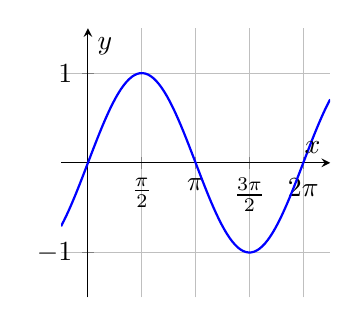
\begin{tikzpicture}
            \begin{axis}[%
                xlabel = {$x$}, ylabel = {$y$},
                xmin = -1 * 0.25 * pi, xmax = (9 * pi) / 4,
                ymin = -1.5, ymax = 1.5,
                xtick = {
                    0, 
                    pi / 2, 
                    pi, 
                    (3 * pi) / 2,
                    2 * pi%
                    },
                xticklabels = {
                    $0$,
                    $\frac{\pi}{2}$,
                    $\pi$,
                    $\frac{3\pi}{2}$,
                    $2\pi$%
                },
                ytick = {
                    -1,
                    1
                },
                axis lines = center, grid = both,
                width = 5cm, height = 5cm,
                trig format plots=rad
            ]
            \addplot[color = blue, thick, domain = -1 * 0.25 * pi:9/4*pi, samples = 100]{sin(x)};
            \end{axis}
        \end{tikzpicture}
    \end{minipage}
    \begin{minipage}[c]{0.66\textwidth}
        At left is the function $f(x) = \sin(x)$ graphed on the $xy$-plane, where $x$ is an angle in radians. There are a few things to note about this function.
        \begin{itemize}
            \item It's not like any function we've seen in the past. It's a wave that goes up and down as it moves along $x$.
            \item It has \textbf{zeroes} at $0$, $\pi$, and $2\pi$. More generally, it has zeroes at $n\pi$, where $n$ is any integer\\
            (i.e. $1,2,3,4,\text{etc.}$)
        \end{itemize}
    \end{minipage}
\end{center}
\begin{itemize}
    \item It has a maximum and minimum value of $1$ and $-1$, meaning the range of this function is $y \in [-1, 1]$. (yet another reason why $r = 1$ is so important).
    \begin{itemize}
        \item Those peaks are reached when $x = \frac{\pi(2n + 1)}{2}$, where $n$ is an integer\\(i.e. $1,2,3,4,\text{etc.}$) This ensures that the numerator is $\frac{\text{odd number} \times \pi}{2}$. Using $2n + 1$ (which guarantees an odd number) is what gets the values 
        $x = \frac{1\pi}{2}, \frac{3\pi}{2}, \frac{5\pi}{2},\dots$
    \end{itemize}
    \item At $x = 2\pi$, it essentially resets to what it was at $x = 0$ (same direction and $y$-value).
    \item It may not look super obvious from the table, but this function continues forever in the positive and negative $x$ directions. This means the domain of $\sin(x)$ is $x \in (-\infty, \infty)$.
\end{itemize}
\clearpage
\section{The Cosine Function}
The cosine function is very similar to the sine function. It's the second of the three basic trigonometric functions. Like the sine function, it takes angles (either in degrees or radians) as an input. But it instead outputs the ratio of the side adjacent to the angle and hypotenuse of a right triangle. This is written as:

\begin{center}
    \begin{minipage}[c]{0.4\linewidth}
        \centering
        \begin{tikzpicture}
            \begin{axis}[%
                xmin = -0.3, xmax = 1.1,
                ymin = -0.3, ymax = 1.1,
                axis lines = none,
                width = \linewidth, height = \linewidth
            ]
            
            \draw[red, thick] (0,0) -- (1,0) node[midway, below, black] {adj};
            \draw[red, thick] (1,0) -- (0,1) node[midway, above right, black] {hyp};
            \draw[blue, thick] (0,0) -- (0,1) node[midway, left, black] {opp};
            
            \node[right] at (0.65, 0.1) {$\theta$};
            \draw[color = black, thick] (0.8,0) arc (180:135:0.2);
            
            \draw[thick, color = black] (0,0.1) -- (0.1,0.1) -- (0.1,0);
            \end{axis}
        \end{tikzpicture}
    \end{minipage}%
    \begin{minipage}[c]{0.3\linewidth}
        \[
            \cos(\theta) = \frac{\text{adjacent}}{\text{hypotenuse}}
        \]
    \end{minipage}
\end{center}
\begin{center}
    \begin{minipage}[c]{0.33\linewidth}
        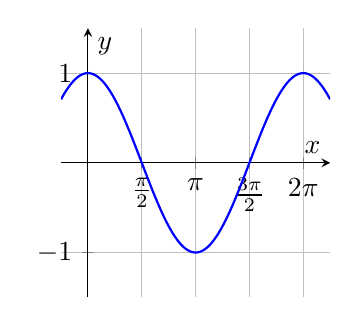
\begin{tikzpicture}
            \begin{axis}[%
                xlabel = {$x$}, ylabel = {$y$},
                xmin = -1 * 0.25 * pi,, xmax = (9 * pi) / 4,
                ymin = -1.5, ymax = 1.5,
                xtick = {
                    0, 
                    pi / 2, 
                    pi, 
                    (3 * pi) / 2,
                    2 * pi%
                    },
                xticklabels = {
                    $0$,
                    $\frac{\pi}{2}$,
                    $\pi$,
                    $\frac{3\pi}{2}$,
                    $2\pi$%
                },
                ytick = {
                    -1,
                    1
                },
                axis lines = center, grid = both,
                width = 5cm, height = 5cm,
                trig format plots=rad
            ]
            \addplot[color = blue, thick, domain = -1 * 0.25 * pi:9/4*pi, samples = 100]{cos(x)};
            \end{axis}
        \end{tikzpicture}
    \end{minipage}
    \begin{minipage}[c]{0.66\textwidth}
        At left is the function $f(x) = \cos(x)$ graphed on the $xy$-plane, where $x$ is an angle in radians. There are a few things to note about this function.
        \begin{itemize}
            \item Like the sine function, it's a wave that goes up and down as it moves along $x$.
            \item It has \textbf{zeroes} at $\frac{\pi}{2}$ and $\frac{3\pi}{2}$. More generally, it has zeroes at $\frac{\pi(2n + 1)}{2}$, where $n$ is any odd integer\\
            (i.e. $1,3,5,7,\text{etc.}$)
        \end{itemize}
    \end{minipage}
\end{center}
\begin{itemize}
    \item It has a maximum and minimum value of $1$ and $-1$, meaning the range of this function is $y \in [-1, 1]$. (yet another reason why $r = 1$ is so important).
    \begin{itemize}
        \item Those peaks are reached when $x = n\pi$, where $n$ is an integer\\(i.e. $1,2,3,4,\text{etc.}$)
    \end{itemize}
    \item Just like the sine function, it essentially resets to what it was at $x = 0$ when it reaches $x = 2\pi$ (same direction and $y$-value).
    \item Also like the sine function, it continues forever in the positive and negative $x$ directions. This means the domain of $\cos(x)$ is $x \in (-\infty, \infty)$.
\end{itemize}
Something you may notice about the cosine function is that it is exactly equal to the sine function if you move it $\frac{\pi}{2}$ units to the right. In other words:
\begin{align*}
    \text{In Radians: } &\sin(\theta) = \cos\left(\theta - \frac{\pi}{2} \right) \\
    \text{In Degrees: } &\sin(\theta) = \cos\left(\theta - 90\right)
\end{align*}